% dynamics/schwerpunkt_state.tex
\chapter{What \emph{Schwerpunkt} Can Mean}
\label{chap:schwerpunkt-state}

\section*{A model reference, not a new canonical state}

The railway state and traversal \(s(t)\) expose a moving vehicle to geometry.
They do not select a vehicle model or a point whose motion represents that
vehicle. The German word \emph{Schwerpunkt} is therefore retained only where
its mathematical role is stated.

\begin{figure}[htbp]
\centering
% figures/dynamics/schwerpunkt_trajectory.tex
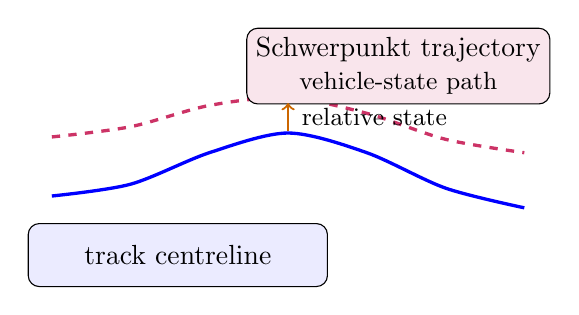
\begin{tikzpicture}[
  x=1cm,y=1cm,
  box/.style={draw, rounded corners, align=center, minimum width=3.8cm, minimum height=0.8cm}
]
\draw[very thick, blue] plot[smooth] coordinates {(0,0) (1,0.15) (2,0.55) (3,0.8) (4,0.55) (5,0.1) (6,-0.15)};
\draw[very thick, purple!80, dashed] plot[smooth] coordinates {(0,0.75) (1,0.88) (2,1.15) (3,1.25) (4,1.05) (5,0.72) (6,0.55)};

\node[box, fill=blue!8] at (1.6,-0.75) {track centreline};
\node[box, fill=purple!10] at (4.4,1.65) {Schwerpunkt trajectory\\\small vehicle-state path};

\draw[->, thick, orange!80!black] (3,0.82) -- (3,1.18);
\node[right] at (3.05,1.0) {\small relative state};
\end{tikzpicture}

\caption{A model-selected reference-point trajectory relative to the railway state; it is not Alignment geometry.}
\label{fig:schwerpunkt-trajectory}
\end{figure}

\begin{principle}[Qualified Schwerpunkt use]
\label{princ:schwerpunkt-principle}
An occurrence of \emph{Schwerpunkt} shall identify its owning subject, model,
reference frame and evidential status. It is not a canonical Kernel state.
\end{principle}

\begin{principle}[Schwerpunkt is not geometry]
\label{princ:schwerpunkt-not-geometry}
Changing or evaluating a model reference-point trajectory does not change
Alignment identity or replace its intrinsic construction.
\end{principle}

\section{Center of mass and reduced reference point}

The physical centre of mass is a property of a particular loaded vehicle.
A reduced vehicle model \(M\), however, may use a reference point \(P_M\)
that coincides with an assumed centre of mass only under stated loading and
rigid-body assumptions. A representative trajectory point, an optimization
aggregate and a conceptual ``focus'' are different objects and shall not be
denoted silently by the same symbol.

\begin{definition}[Model-qualified reference-point state]
\label{def:cg-state}
For vehicle subject \(V\), response model \(M\), frame \(F\), qualified
railway state \(S_{\mathrm{rail}}\), traversal \(s(t)\), parameters \(Q_M\)
and initial conditions \(I_M\), the predicted reference-point state is
\[
x_{P_M}^{\mathrm{pred}}(t)
=
\mathcal D_M(S_{\mathrm{rail}}(s(t)),Q_M,I_M)_{{P_M},F}.
\]
It is a model output with the provenance and validity of those inputs. It is
neither an observation nor proof of the physical centre-of-mass motion.
\end{definition}

\begin{definition}[Center-of-gravity trajectory]
\label{def:cg-trajectory}
The notation \(x_{\mathrm{CG}}(t)\) may be used only when \(P_M\) has explicitly
been identified with the modelled centre of mass. Otherwise
\(x_{P_M}(t)\) is used.
\end{definition}

\section{What may be derived}

\begin{definition}[Operational balance]
\label{def:operational-balance}
Operational balance in this chapter means a declared model relation evaluated
in a declared frame. It is not a generic vehicle condition.
\end{definition}

\begin{definition}[Balance trajectory]
\label{def:balance-trajectory}
A balance trajectory is the time- or station-dependent result of that
relation, with its model, frame, signs, velocity and cant assumptions attached.
\end{definition}

\begin{definition}[Effective operational acceleration]
\label{def:effective-operational-acceleration}
In the reduced track-frame test used in \cref{chap:dynamic-balance},
\(a_{\mathrm{eff}}=v^2\kappa-g\sin\phi\) is a residual indicator. It is not
the acceleration of \(P_M\) unless a response model establishes that mapping.
\end{definition}

\begin{definition}[Roll evolution]
\label{def:roll-evolution}
Roll evolution is a response-model output requiring inertia, suspension,
loading, initial conditions and a frame convention; cant alone does not
determine it.
\end{definition}

\begin{definition}[Operational comfort]
\label{def:operational-comfort}
Comfort is a purpose- and rule-qualified evaluation of applicable evidence.
Neither a reference-point trajectory nor a reduced balance residual is by
itself a comfort statement.
\end{definition}

\begin{definition}[Operational trajectory shaping]
\label{def:trajectory-shaping}
Trajectory shaping is an optimization description only after variables,
constraints, response model and objective have been declared. Its result is a
candidate.
\end{definition}

\section{Schwerpunkt interpretation and realization}

A target Alignment, its Metric Realization, a constructed asset, an
observed-state estimate and a predicted reference-point response remain
separate. A model may consume a qualified realization or an observed-state
estimate, but the output inherits its uncertainty and applicability. The
phrase \emph{Schwerpunkt-Trassierung} is consequently historical or
illustrative shorthand for model-qualified reference-point trajectory
investigation; it names neither a Kernel concept nor a current AXTRAN
capability.

\section{Claim status}

\begin{center}
\small
\begin{tabular}{p{0.28\linewidth}p{0.25\linewidth}p{0.38\linewidth}}
\toprule
Expression & Status & Defensible use\\
\midrule
physical centre of mass & physical/model parameter & particular vehicle and loading\\
\(P_M\) trajectory & model prediction & identified \(M,F,Q_M,I_M\)\\
Schwerpunkt State & non-canonical shorthand & only with the preceding qualification\\
Schwerpunkt optimization & candidate & declared optimization problem only\\
\bottomrule
\end{tabular}
\end{center}

The next chapter uses the simplest residual relation deliberately. Its
limitations show why a model output cannot become an evaluation or decision
merely by receiving a state-like name.
